\scanpage{99}
% archive foliation: 101
\uline{Résumé} Cas $E_a$ :
\[
\left\{\begin{array}{l}
\text{base }u=e_0,\ v=e_1\\
\text{forme }\deleted{Q(e_0)=Q(e_1)}\quad Q(xe_0+ye_1)=x^2+ay^2
\end{array}\right.
\]
Si on \unsure{met|veut} la forme $Q$ sous forme standard on
prend la \inserted{nouvelle} base
$\underbrace{e_0}_{1},\underbrace{\frac1{\sqrt a}e_1}_{i}$, on trouve donc la base
$1,\sqrt a\,i$ d'où
\[\boxed{\tau=\sqrt a\,i},\]

Cas $E'_a$ : base, \deleted{$\unsure{u=e_0,v=\frac12u|u=e_0,v=u}$}
distinguée p.r. à $Q$ les
\[
e_0=u,\quad e_1=2v-u;\qquad Q(xe_0+ye_1)=x^2+ay^2
\]
\[v=\frac12(e_0+e_1).\]
\unsure{au|on} \deleted{\unsure{premier}} changement de base.
\[
\underbrace{e_0}_{1},\underbrace{\frac1{\sqrt a}e_1}_{i}
\qquad\text{bien orthonormale}
\]
et on a $u\Rightarrow1$, $v\mapsto\frac12(1+\sqrt a\,i)$, donc
\[\boxed{\tau=\frac12(1+\sqrt a\,i)}=\frac12+\frac{\sqrt a}{2}i.\]
\figure{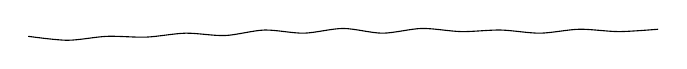
\begin{tikzpicture}\draw plot[smooth]coordinates{(0,0)(.5,-.05)(1,0)(1.5,-.01)(2,.04)(2.5,.01)(3,.08)(3.5,.04)(4,.1)(4.5,.04)(5,.1)(5.5,.06)(6,.08)(6.5,.04)(7,.09)(7.5,.06)(8,.09)};\end{tikzpicture}}

Calcul du groupe des pts réels d'une courbe $E_a$, $E'_a$.

Pts réels sont les $x\bmod\pi$ ($x\in\pi_{\mathbb R}$) tels que
\[\sigma x\equiv x\quad(\pi)\]
\uline{Distinguons les deux cas}.

1) $\uline{E_a}$ \deleted{$\sigma(e_0,e_1)=$} $\sigma(x,y)=x,-y$
\[\text{donc}\qquad\sigma(x,y)-(x,y)=(0,2y)\]
donc la condition est que $2y\in\mathbb Z$. Donc il y a \deleted{\unsure{les}}
les pts de $\deleted{\unsure{\frac02}}\mathbb R e_0$ et de
$\deleted{\mathbb R}(0,\frac12)+\mathbb R e_0$, donc
\uline{deux composantes connexes} \deleted{pour} $X(\mathbb R)$.

\margin{$\unsure{<}$}
